\section{Results and Discussion}
\subsection{RHESSI Hard X-rays}
%RHESSI
For a sunquake to be generated by accelerated paticle collision then the incident beam must be aligned over the acoustic impact location \citep{1998IAUS..185..191K}. To highlight this spatial alignment, RHESSI 50 to 100 keV HXR and sunquake egression power contours are plotted on a reverse colour, filtered HMI continuum image shown in figure \ref{hmicontext}. The contours show a reasonable alignment but a more rigorous way to test the spatial and temporal relationship between nonthermal electrons, sunquake and other emission is to analyse lightcurves from the region of interest.   %explain alignment of different faetures and the significance      

RHESSI HXR data is taken from central coordinates 518" by 262", sampling the sunquake epicenter. When this data is fit to a nonthermal electron model a spectrum is produced, which can be used to plot the energy curve shown in Figure \ref{erhessi}. The plot shows 10 - 100 keV HXR power as a function of time. The impulsive phase of the flare is visible from 17:46, peaking at 17:47, with the plot showing a double peak profile which climbs from $1.0{\times}10^{28}$ to $2.5{\times}10^{29}$ erg. To put this in the context of the associated sunquake, the HXR power can be used to estimate the amount of energy provided to the acoustic impact area, or nonthermal flux via

\begin{equation}\label{electronflux}
F_e = \frac{P_{e}}{A_{HXR}}
\end{equation}

where flux $F_e$ is in units of erg.s$^{-1}$.cm$^{-2}$, $P_e$ is nonthermal power and the HXR emission area is determined by the $90\%$ HXR contour in Figure \ref{hmicontext}, rendering $A_{HXR} \sim \pi (2"{\times}7.25{\times}10^{7})^{2} = $ 6.61{\times}10^{16}$ cm$^{2}$. The resulting flux turns out to be $F_e \sim 10^{44}$ which when multiplied by the sunquake area, can provide an upper limit for the nonthermal power available for generating an acoustic disturbance $P_{e}(A_{sqk}) = \frac{F_e}{A_{sqk}}$. So using the available nonthermal energy, $P_e \sim 2.5{\times}10^{29}$ erg.s$^{-1}$ and $A_{sqk} \sim 2.6{\times}10^{16}$ $cm^{2}$. $P_{e}(A_{sqk}) \sim 10^{28}$ and when compared with the sunquake power $P_{sqk} \sim 1.3\pm0.05{\times}10^{26}$ $erg.s^{-1}$ it is clear that the electron beam does have the required 1000 times more energy required to the sunquake. Another interesting quantity to investigate is the momentum of the particle beam. Electron momentum can be calculated by 


\begin{equation}\label{electron-momentum}
p_e=\tau \sqrt{2m_e} P_{e}
\end{equation}

where $m_e$ is electron mass, $\tau$ is the time duration of flare impulsive phase and $P_{e}$ is described by equation \ref{pnth1}. Substituting values in to equation \ref{electron-momentum} yields an electron momentum of $p_e \sim 1.35{\times}10^{17}$ g cm s$^{-1}$. Assuming the energy in the electron beam is equal to that in a population of accelerated protons \citep{2000ApJ...542..513E}, then calculation of a theoretical proton beam momentum, where $m_p$ is the proton mass, is by the relation,

\begin{equation}\label{proton-momentum}
p_p \sim p_e \sqrt{\frac{m_p}{m_e}}
\end{equation}

Which yields a proton momentum of $p_p \sim 5.79{\times}10^18$ g cm s$^{-1}$, an order of magnitude greater than $p_e$. This is because $m_p ~ 2000m_e$ meaning the square root in equation \ref{proton-momentum} renders the result $p_p \sim 44.7p_e$. So in order to determine whether a particle beam carries enough momentum to stimulate a sunquake, a calculation of the momentum needed to initiated the acoustic response is required.\\

The momentum needed to produce the sunquake is

\begin{equation}
p_{sqk}\sim \rho \; l^{3} \; v
\end{equation}\label{sqk-momentum} 

where all terms are tailored for photospheric values, hence density $\rho \sim 10{-8}$g cm$^{-3}$; sound speed $v \sim 10^{6}$ cm.s$^{-1}$. The length-scale, $l \sim  1.82{\times}10_{8}$, corresponds to the sunquake impact diameter, 

\begin{equation}
l = 2\sqrt{\frac{A_{sqk}}{\pi}}
\end{equation}\label{lengthscale}

Equation \ref{sqk-momentum} gives the momentum of the acoustic reponse as $p_{sqk} = 6.03{\times}10^{22}$ g cm s$_{-1}$, which when compared to particle beam momenta, $p_e$ and $p_p$, is $10{5}$ and $10^{4}$ times larger respectively. This means that even if an electron or proton beam can make it down to the photosphere, it wouldn't have the necessary momentum to cause the sunquake on it's own. In reality, calculated momenta are idealistic, not treating the effects of energy loss due to energy dissapation. The point being that for a particle beam to make it to the photosphere, it has to traverse 9 pressure scale heights, increasing in density with depth. As density increases particles in the beam are more likely to encounter ambient plasma, and as a result are deccelerated, giving up as energy as emission. So if or when the beam reaches the photosphere, much of it's energy and momentum has already been dissapated in the chromosphere, making the generation of a sunquake via just the particle beam even more unlikely.

\begin{figure}[H]
  \begin{center}
  \textbf{RHESSI 10 - 100 keV Hard Xray Energy Over Time}\par\medskip
  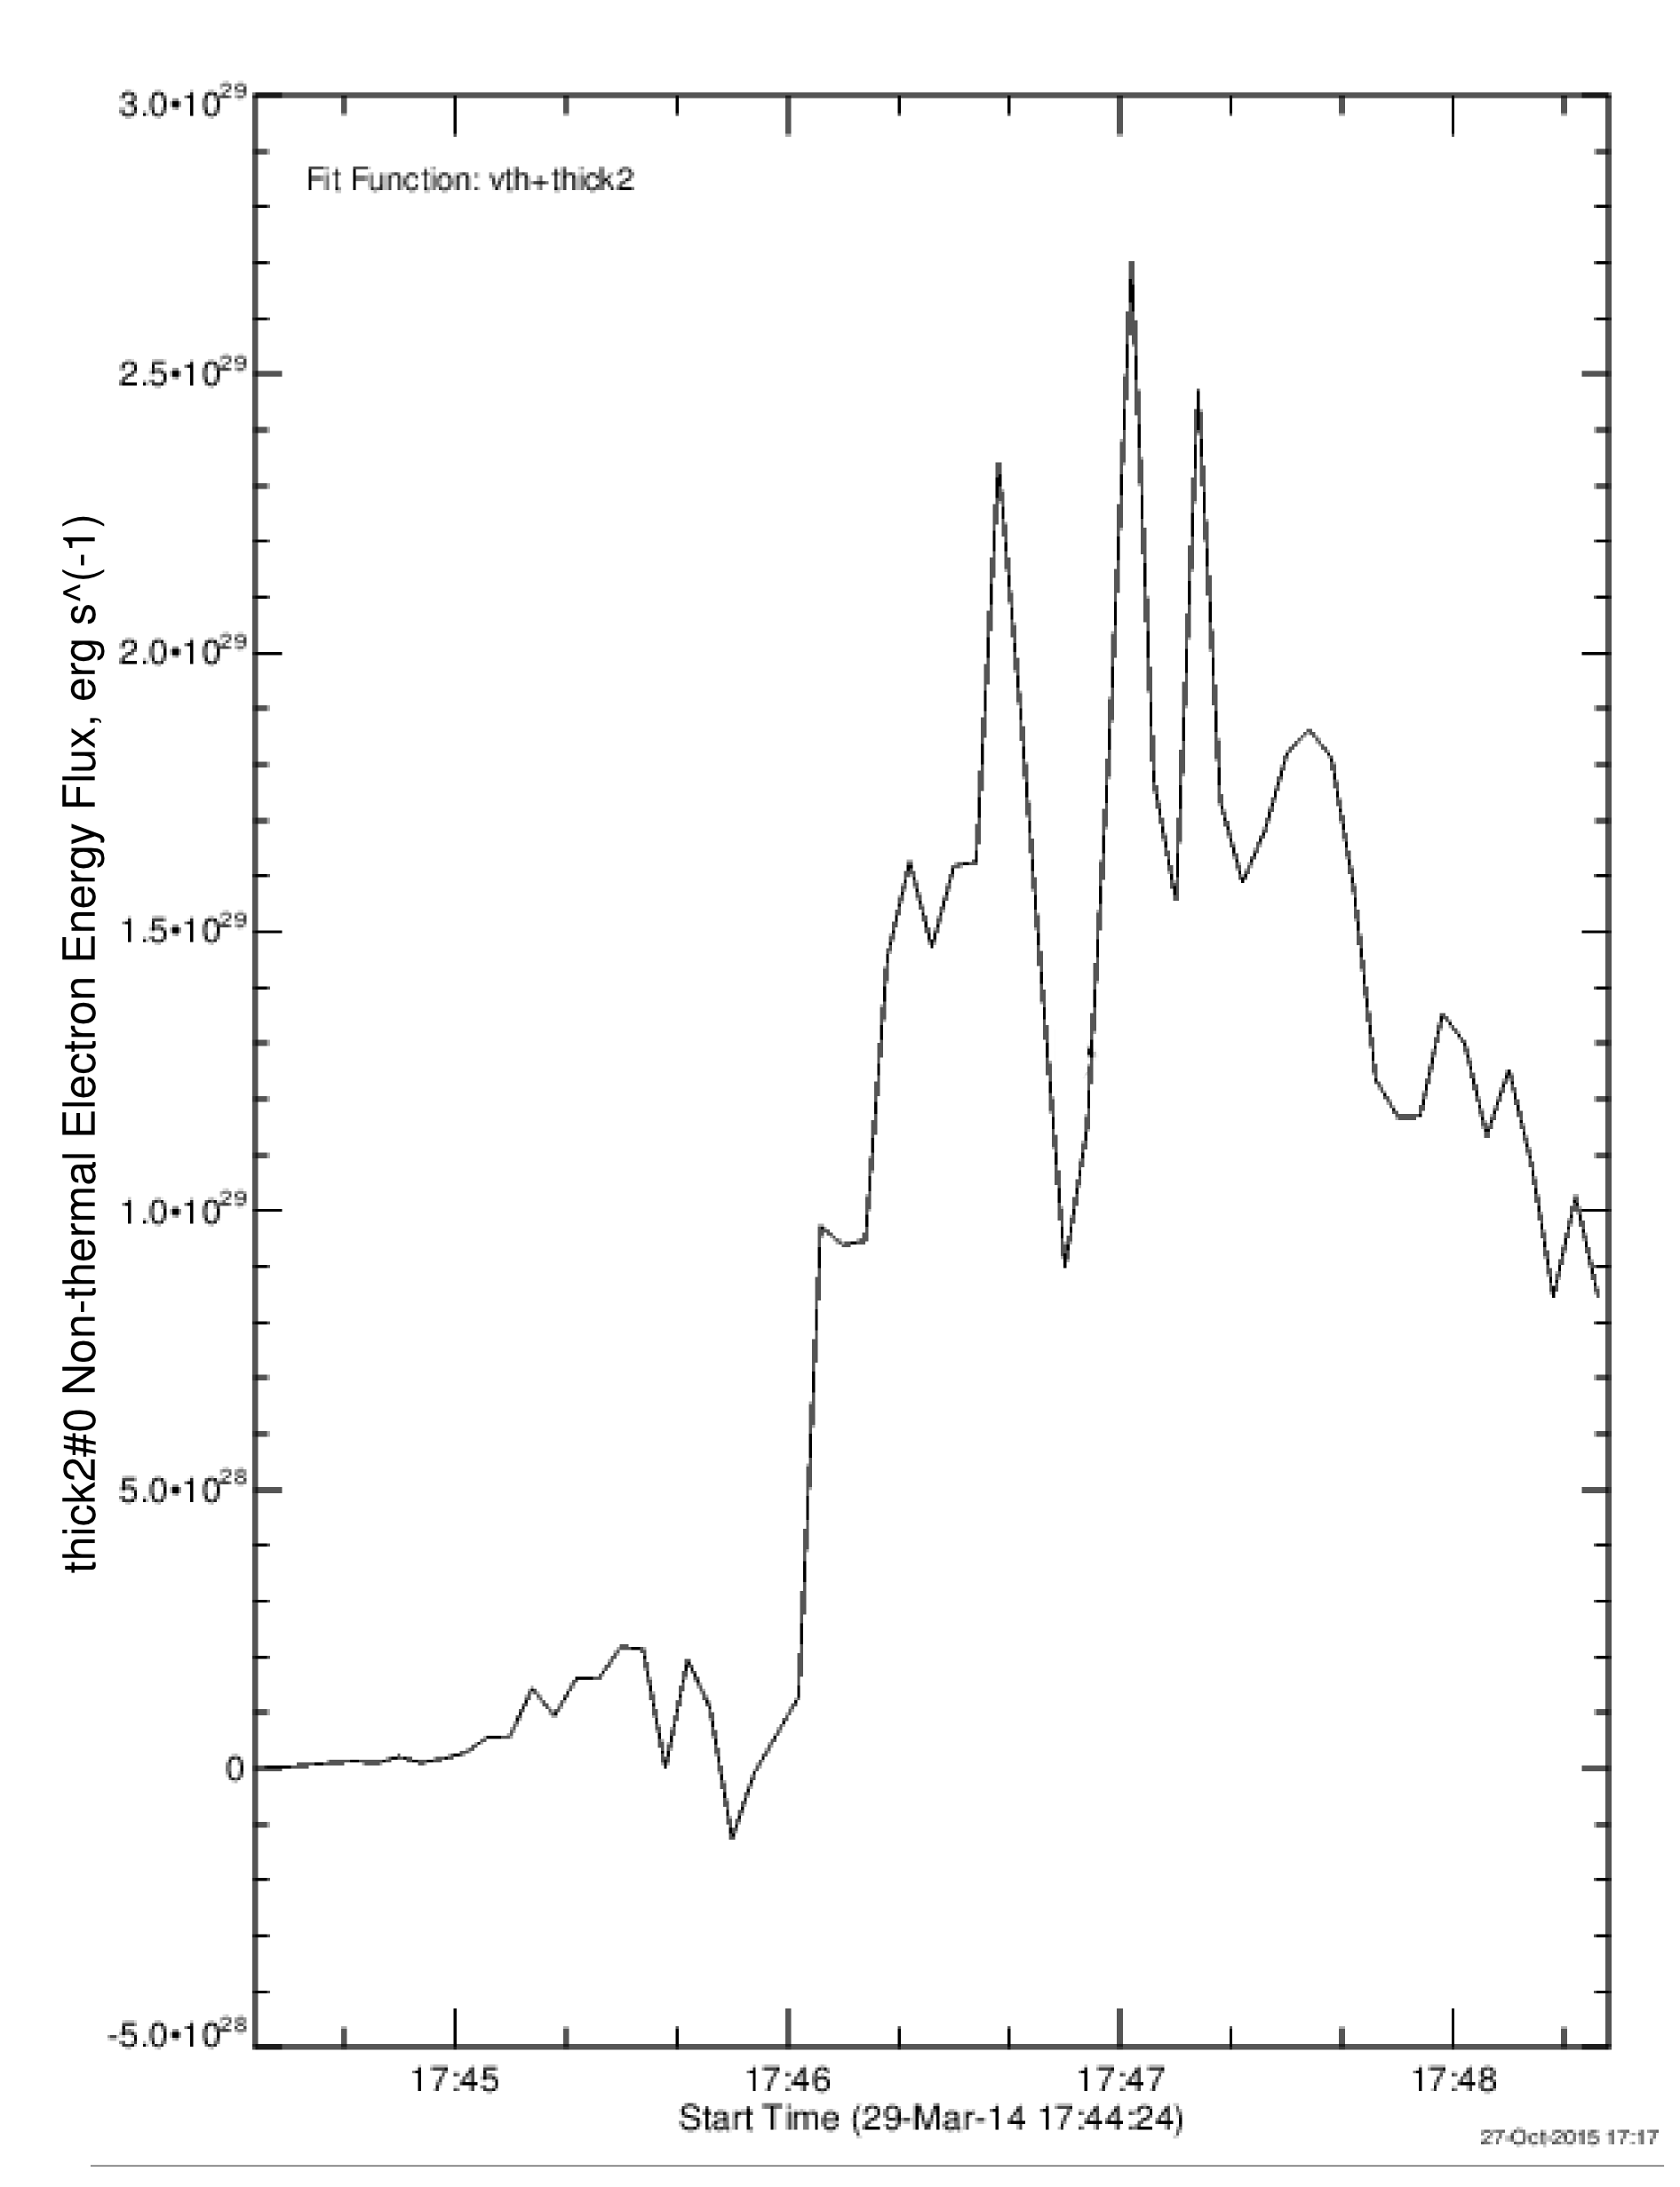
\includegraphics[width=0.6\textwidth]{rhessi-energy-curve}
  \end{center}
  \caption{Shows the energy evolution of hard x-ray emission collected by RHESSI 10 to 100 keV bins over the sunquake region (518", 262"). HXR emission is due to non-thermal electrons, thus energy is calculated by fitting data to the collisional thick target model. The HXRs impulsive phase begins at around 17:46 and peaks at 17:47, showing temporal alignment with IRIS and HMI datasets shown if Figure \ref{fluxladder}}
\end{figure}\label{erhessi}

\subsection{Emission Captured By IRIS and HMI}
%Si IV, Mg II, Balmer, MG II w, HMI
However, energy deposited into the atmosphere by the particle beam can lead to other sunquake generation mechanisms, such as radiative backwarming and shocks which are described in sections \ref{sunprog}. A recent result from \cite{2016ApJ...816...88K} shows that the intensity of Balmer continuum observed in this event could come from either; 23\% of nonthermal electrons with energy $<20$ keV; or the entire population of nomthermal electrons with energy $<40$ keV. This means that a large portion of energy delivered to the lower atmosphere by the electron beam is dissapated causing various continua and emission lines. Shown in Figure \ref{fluxladder} are lightcurves of emission from the lower solar atmosphere, captured by IRIS and SDO HMI. From top to bottom the plot shows data from IRIS SJ Si IV, IRIS SJ Mg II, IRIS SG Balmer Continuum, IRIS SJ Mg II wing and SDO HMI visible continuum sampled from six coordinates in the flare ribbon. Si IV and Mg II IRIS SJ data, show a distinct cutoff which is caused by over saturation of the instrument CCD, meaning flux measurements during the impulsive phase are a lower estimate. However, Si IV and Mg II lightcurves can still be used to confirm temporal and spatial alignment of energy deposition at these wavelengths. All coordinates in all datasets show a synchronised impulsive peak, with the exception of MG II wing where only coordinates four and five exhibit a siginifcant enhancement. The red solid line in each data set is sampled from the sunquake location. At first glance the sunquake location in the plots does not seem to have any obvious differences other than a slight time delay in peak Balmer continuum emission. The delay appears to be around 45 seconds after the impulsive phase peak at approximately 17:48 which coincides with the sunquake onset time \citep{2015ApJ...812...35M}. Mg II wing data shows no enhancement over the sunquake location. HMI continuum shows significant enhancement over the sunquake, which is aligned in time with the impulsive phase. 




%LADDER PLOTS
\begin{figure}[H]
  \begin{center}
  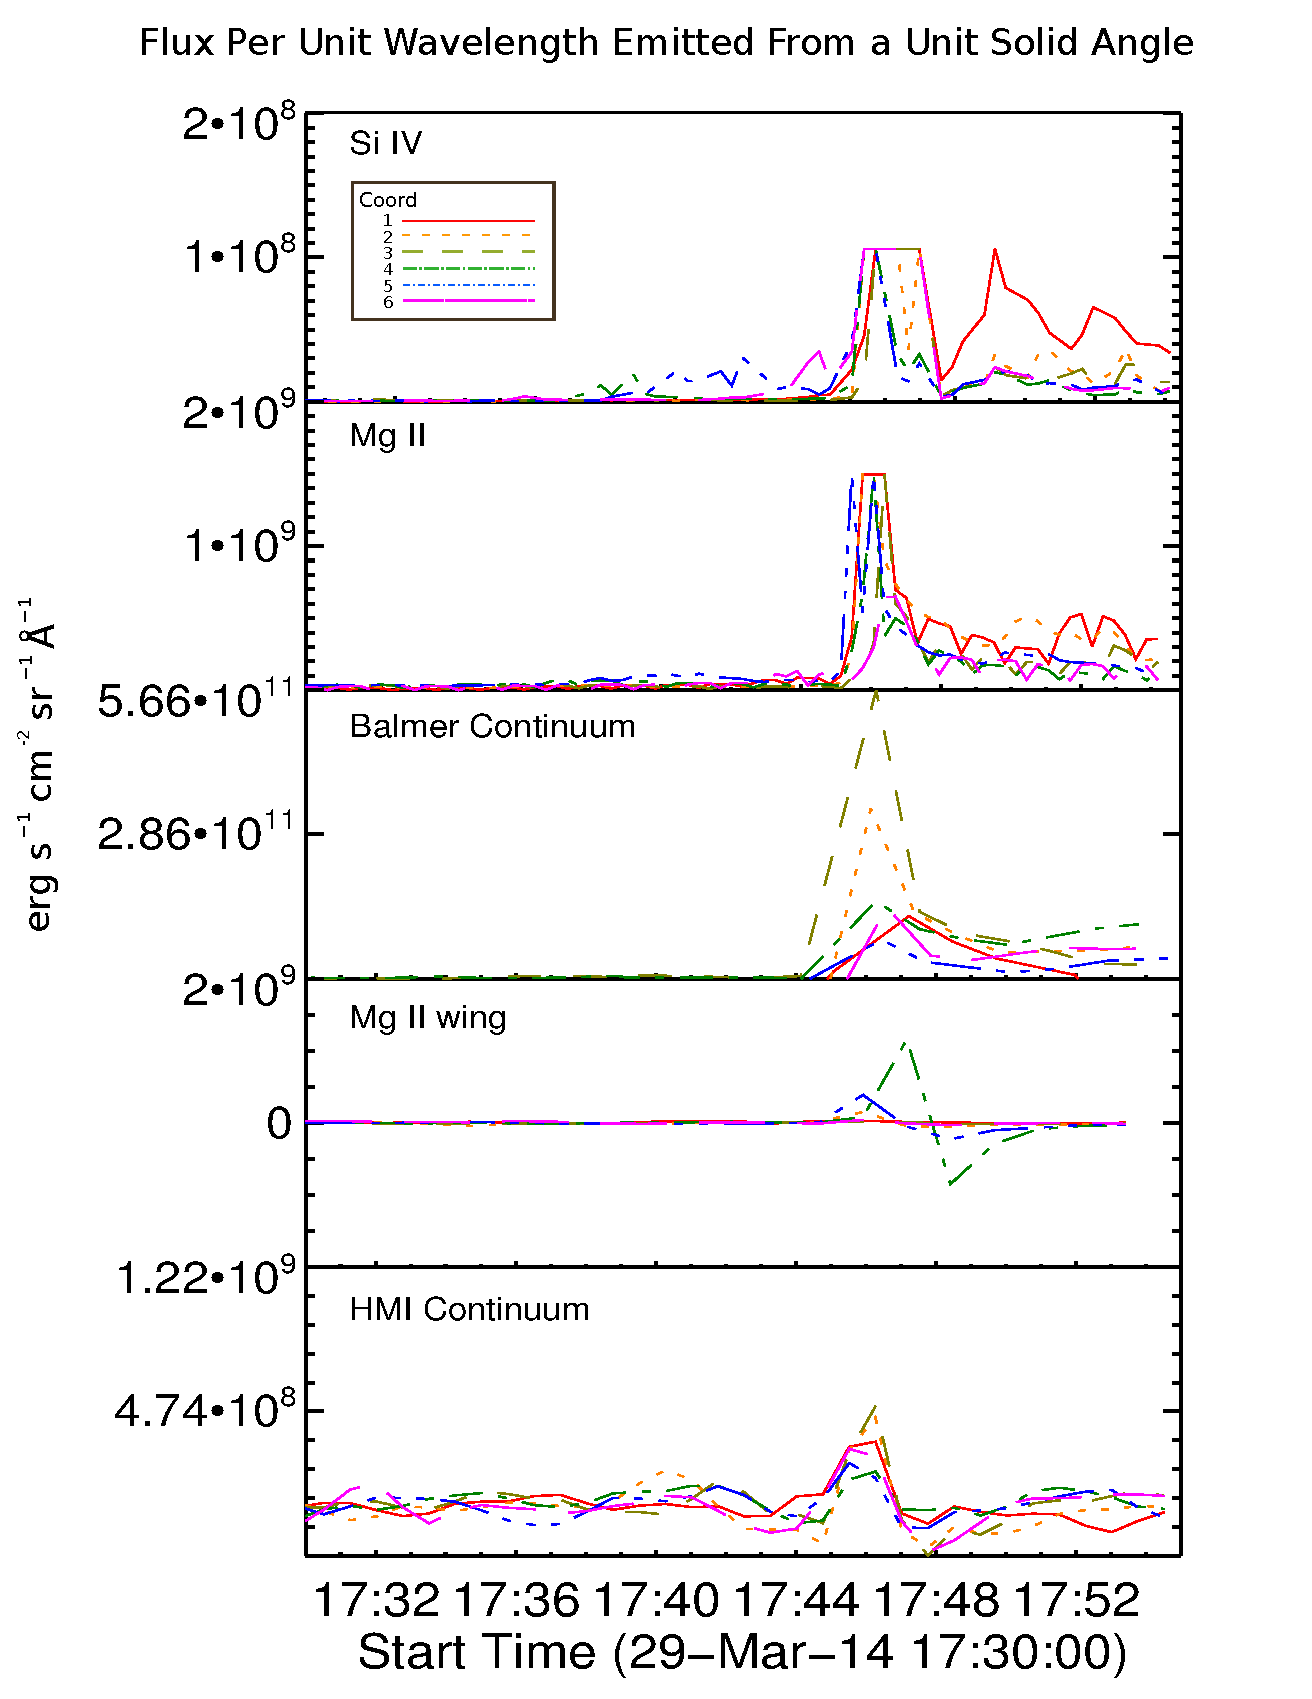
\includegraphics[width=0.6\textwidth]{29-Mar-14-Flux-Ladder}
  \end{center}
  \caption{Shows flux per wavelength from a unit solid angle or intensity. The six lines (see legend) represent areas centered on regions 1 to 6, relating to heliocentric coordinates shown in Table \ref{coordtab}. The solid red line is directly over the sunquake location. Each plot represents an independant data set, in order from top to bottom the sets are; IRIS SJ 1400 (Si IV); IRIS SJ 2796 (Mg II); IRIS SG  2825.7 to 2825.8 (Balmer Continuum); IRIS SJ 2832 (Mg II wing); SDO HMI continuum}\label{fluxladder}
\end{figure}




\begin{figure}[H]
  \begin{center}
  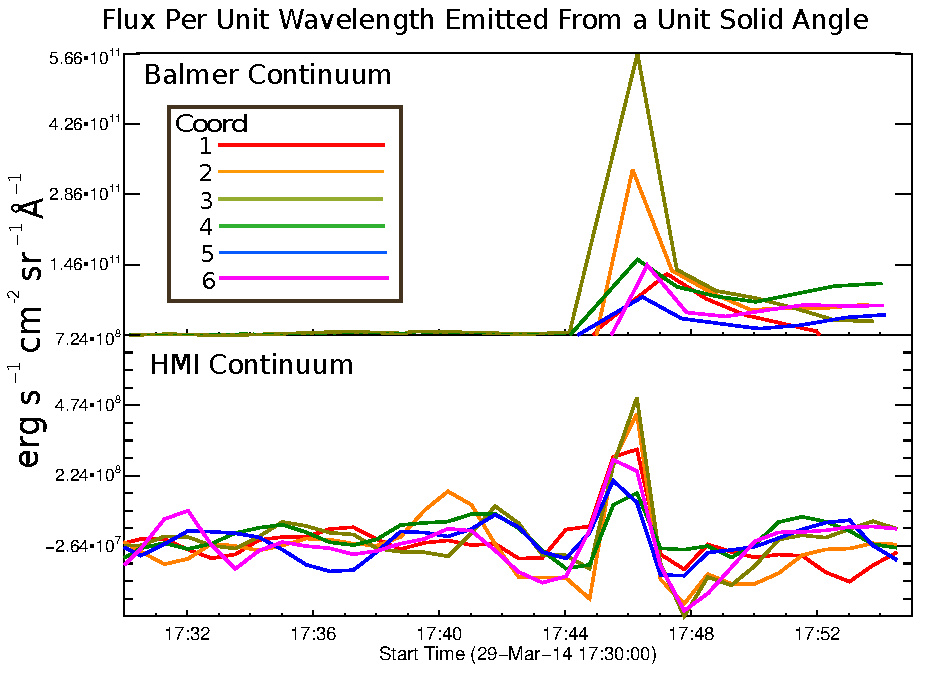
\includegraphics[width=0.6\textwidth]{29-Mar-14-Flux-Ladder-Balm-HMI-Only}
  \end{center}
  \caption{Shows flux per wavelength from a unit solid angle. The six lines (see legend) represent areas centered on regions 1 to 6, relating to heliocentric coordinates shown in Table \ref{coordtab}. The solid red line is directly over the sunquake location. Each plot represents an independant data set, in order from top to bottom the sets are; IRIS SJ 1400 (Si IV); IRIS SJ 2796 (Mg II); IRIS SG  2825.7 to 2825.8 (Balmer Continuum); IRIS SJ 2832 (Mg II wing); SDO HMI continuum}\label{fluxladder-balm-hmi-only}
\end{figure}


The flux values for Balmer and HMI continuum shown in Figure \ref{fluxladder-balm-hmi-only} can be used to estimate the power of the radiative backwarming. The key being whether the radiative backwarming is powerful enough to generate the white light flare and hence the sunquake. The power profiles shown in Figure \ref{powerladder-balm-hmi-only} are calculated by assuming a homogenous energy distribution in the region surrounding each coordinate, it is then possible to use the relation,

\begin{equation}
P_{Balm} = F_{Balm} \; A_{sqk}  
\end{equation}\label{Pbalm}

where $P_{Balm}$ is the power of the Balmer continuum emitted from an area equal to the sunquake, $A_{sqk}$. The same data set and coordinate scheme is followed as in Figure \ref{fluxladder-balm-hmi-only}. The Balmer continuum over the sunquake shows an impulsive power $P_{Balm} = 6{\times}10^{13}$ erg.s$^{-1}$ which is thirteen orders of magnitude smaller than the power of the sunquake $P_{sqk} \sim 1.3\pm0.05{\times}10^{26}$ $erg.s^{-1}$. This means that there is not enough energy per second deposited by radiative backwarming to create the sunquake. The HMI continuum power, $P_{HMI}$, over the sunquake location peaks at $P_{HMI} = 2{\times}10^{14}$ erg.s$^{-1}$cm$^{-2}$, which is twelve orders of magnitude less than the $P_{sqk}$ but ten times greater than the Balmer continuum. One of the biproducts of radiative backwarming are white light flares in the photosphere. Balmer continuum radiated outward to the observer, is supposed to be equal in power to that emitted downward \citep{1989SoPh..124..303M}. In that case the white light flare shown in the HMI continuum in Figure \ref{powerladder-balm-hmi-only} is only provided $10\%$ of its power by radiatve backwarming. So radiative backwarming at first glance may not be causing the observed white light emission. However, another way to investigate the energy deposition in the lower atmosphere is by integrating radiative flux over the impulsive phase of the flare. This provides an upper limit for the total flux injected into the system during the impulsive phase, which can be used to calculate the total emission power. The integrated flux is calculated,

\begin{equation}
F_{imp} = \int_{0}^{\tau} F(t) \; dt = F(t) \; \tau
\end{equation}\label{f-imp}
 
where the duration of the impulsive phase $\tau = $ and $F(t)$ is the emitted flux at time $t$. The total power emitted during the impulsive phase, $F_{imp}$ is

\begin{equation}
P_{imp}=F_{imp} \; A_{sqk}
\end{equation}\label{e-imp}

where it is assumed that a homogenous energy distribution exists throughout the sunquake impact area. This produces values for each data set tabulated in Table \ref{eimp}. Balmer and HMI continua are the data sets that show the highest integrated energy levels, with comparable values at each coordinate. The fact that Balmer and HMI continua show such similar energies emitted over the impulsive phase means that radiative backwarming is likely causing the white light flare in the photosphere as described in section \ref{wlf}. The highest energy reading in the HMI continuum is over the sunquake, with a value of $1.42{\times}10^{16}$ erg whereas in the Balmer continuum the highest is coordinate three with $2.52{\times}10^{16}$, both of which are ten orders of magnitude smaller than $P_{sqk}$. Meaning that the radiative backwarming mechanism in this case is not powerful enough to produce the sunquake.    


%\begin{figure}[H]
%  \begin{center}
%  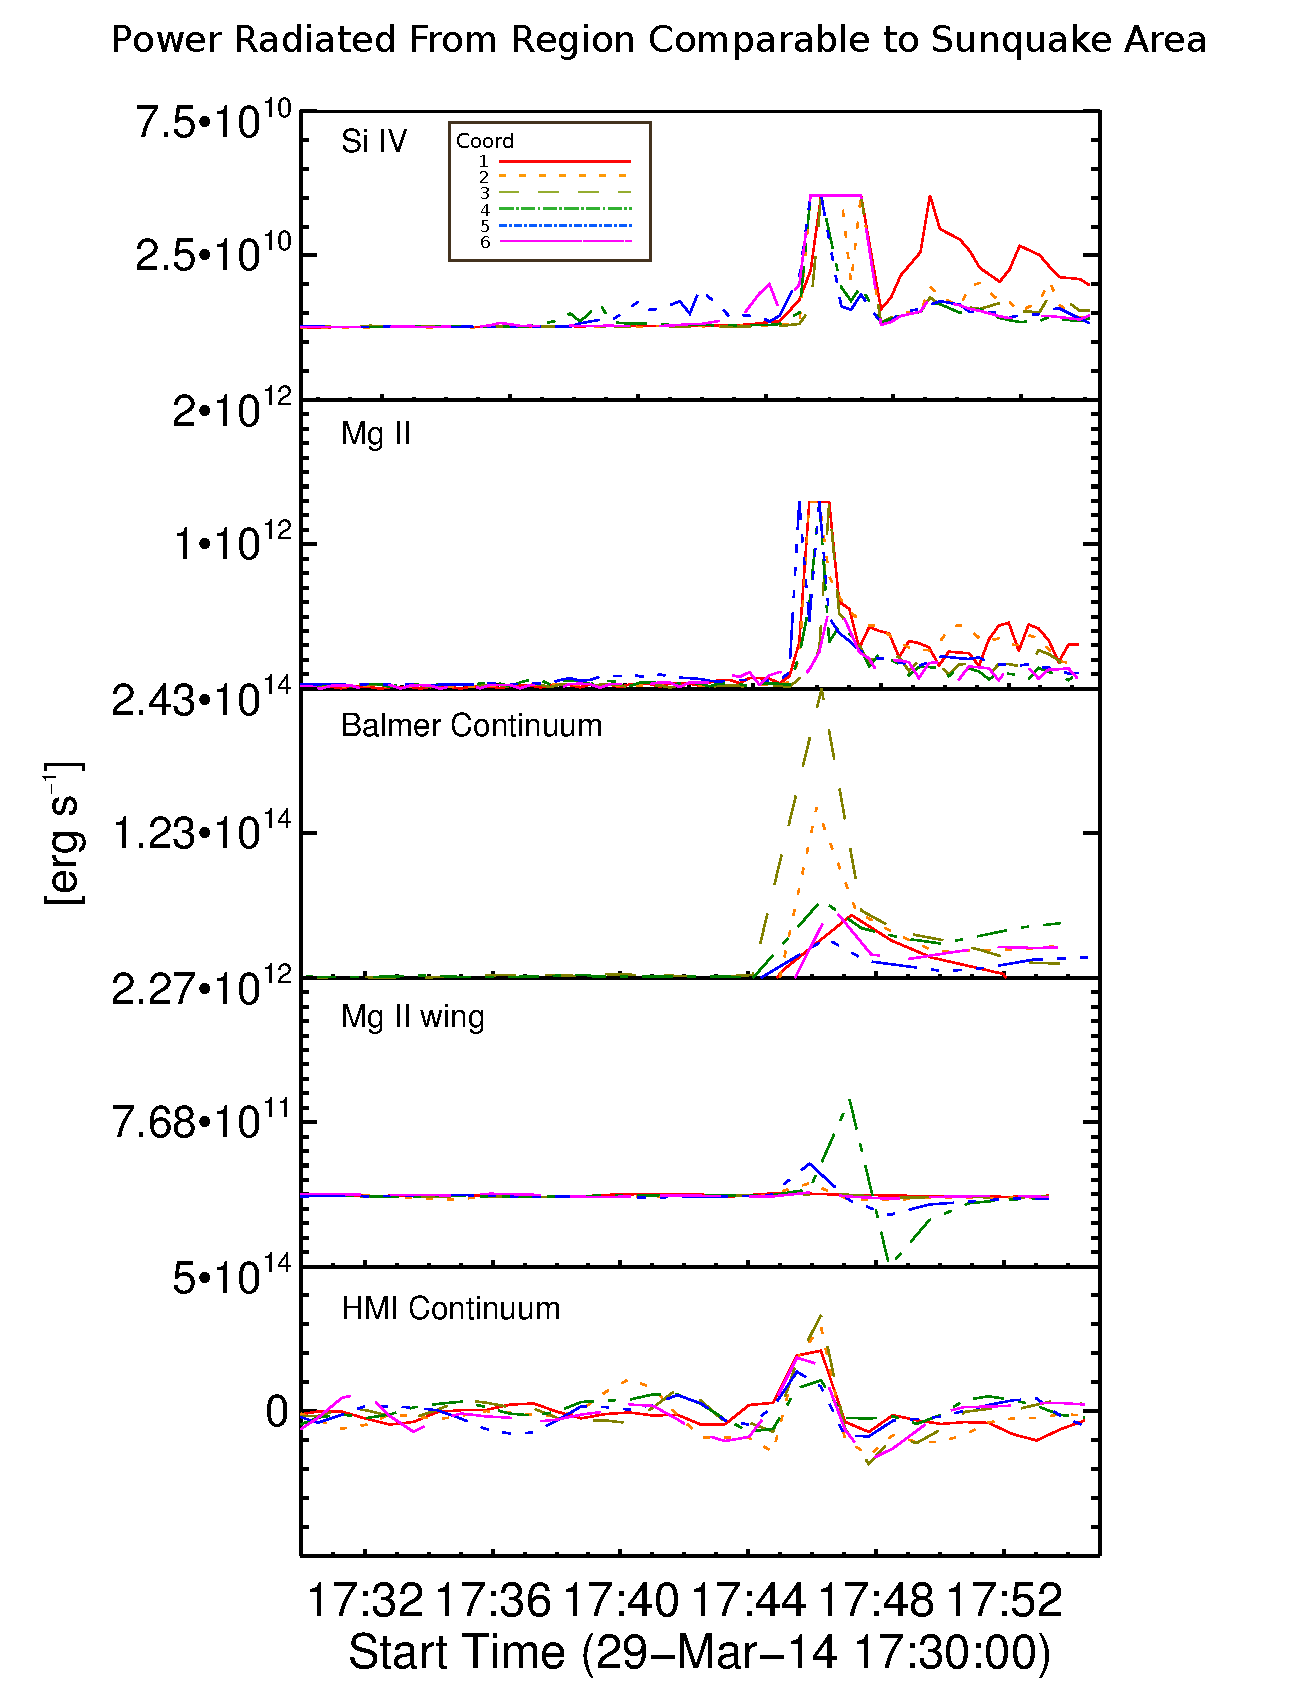
\includegraphics[width=0.6\textwidth]{29-Mar-14-A_sqk-Power-Ladder}
%  \end{center}                                                                                                                                                                                                                                                                                                                                                                                                                                                                                                                                                                                                                                                                                                                                                                                                                                                                                                                                                                                                                                                                                                                                                                                                                                                                                                                                                                                                                                                                                                                                                                                                                                                                                                                                                                                                                                                                                                                                                                                                                                                                                                                                                                                                                                                                                                                                                                                                                                                                                  
%  \caption{Shows radiative power [erg.s$_{-1}$], which is the result of flux data that has been multiplied by the sunquake impact area. The six lines (see legend) represent areas centered on regions 1 to 6, relating to heliocentric coordinates shown in Table \ref{coordtab}. The solid red line is directly over the sunquake location. Each plot represents an independant data set, in order from top to bottom the sets are; IRIS SJ 1400 (Si IV); IRIS SJ 2796 (Mg II); IRIS SG  2825.7 to 2825.8 (Balmer Continuum); IRIS SJ 2832 (Mg II wing); SDO HMI continuum (HMI).}\label{powerladder}
%\end{figure}

\begin{figure}[H]
  \begin{center}
  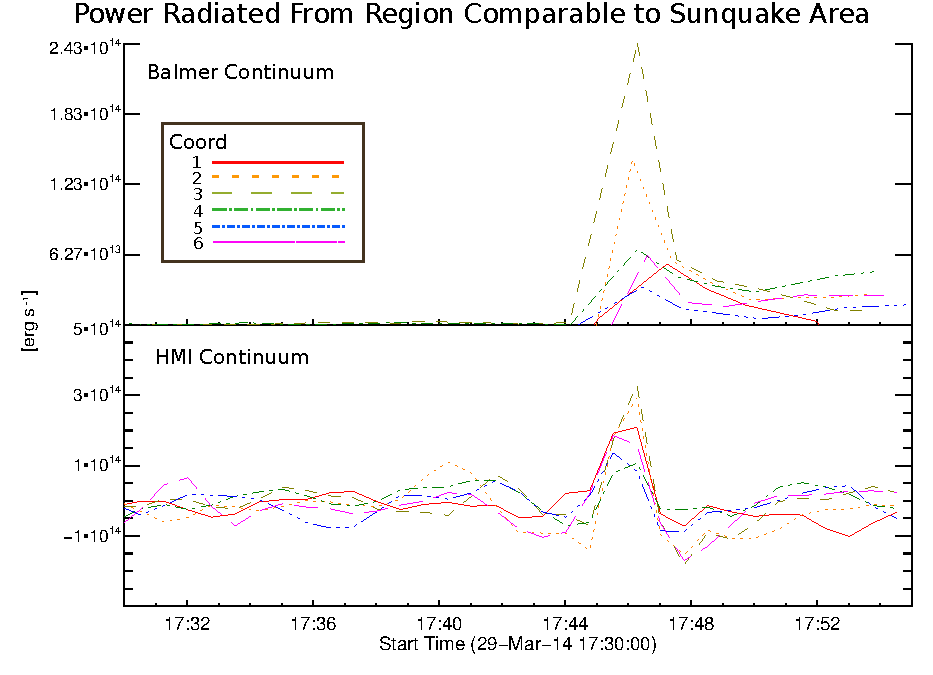
\includegraphics[width=0.6\textwidth]{29-Mar-14-A_sqk-Power-Ladder-Balm-HMI-Only}
  \end{center}
  \caption{Shows radiative power [erg.s$_{-1}$], which is the result of flux data that has been multiplied by the sunquake impact area. The six lines (see legend) represent areas centered on regions 1 to 6, relating to heliocentric coordinates shown in Table \ref{coordtab}. The solid red line is directly over the sunquake location. The top plot is IRIS SG  2825.7 to 2825.8 Balmer Continuum and the bottom plot is SDO HMI continuum.}\label{powerladder-balm-hmi-only}
\end{figure}




\begin{table}[h]
%\tiny
\centering
\begin{tabular}{|c|c|c|c|c|c|c|c|c|c|c|}
Coord Number & Coorinates (x,y) [arcsecs] & $E_{Si IV}$ [erg] & $E_{Mg II}$ [erg] & $E_{Balm}$ [erg] & $E_{Mg II w}$ [erg] & $E_{HMI}$ [erg]\\
\hline
1 & 518.22, 262.00 & 6.74E+12 & 1.41E+14 & 5.98E+15 & 4.27E+12 & 1.42E+16\\
2 & 520.22, 263.00 & 5.65E+12 & 1.35E+14 & 1.71E+16 & 7.14E+12 & 1.10E+15\\
3 & 522.21, 262.00 & 5.18E+12 & 7.83E+13 & 2.52E+16 & 2.91E+12 & 4.82E+15\\
4 & 522.21, 265.00 & 3.93E+12 & 8.35E+13 & 9.89E+15 & 6.70E+13 & 1.28E+15\\
5 & 524.26, 265.00 & 3.98E+12 & 1.03E+14 & 4.37E+15 & 1.86E+13 & 8.99E+14\\
6 & 526.25, 263.82 & 6.91E+12 & 6.34E+13 & 5.24E+15 & 1.74E+12 & 9.88E+14\\
\end{tabular}
\caption{Flux integrated over the flare impulsive phase (17:44 to 17:48) is then multiplied by the sunquake impact area to produce a total deposited energy in erg. The values show are for ribbon sample locations 1 to 6.}\label{eimp}
\end{table}




